\section{Clustering}

\begin{defi}{Clusteranalyse}
    Die \emph{Clusteranalyse} findet Gruppen (\emph{Cluster}) ähnlicher Datenpunkte, ohne dass Labels vorliegen müssen.

    \emph{Clustering} ist also Partitionierung (Einteilung) der Datenpunkte in Gruppen.

    Viele Clusteranalyseverfahren existieren und unterscheiden sich:
    \begin{itemize}
        \item in der Definition von Ähnlichkeit,
        \item in der Definition von Gruppen (Clustern),
        \item im algorithmischen Vorgehen.
    \end{itemize}

    Es gilt:
    \begin{itemize}
        \item Clusteranalyseverfahren finden immer Cluster in den Daten.
        \item Verschiedene Verfahren liefern verschiedene Cluster für dieselben Daten.
        \item Cluster-Verfahren interpretieren die Daten hinsichtlich der den Verfahren (teils implizit) zugrundeliegenden Annahmen.
        \item Wie Clusterings bewertet werden können (also z.B. als sinnvoll bzw. nicht sinnvoll eingestuft werden können), ist aktuelles und im Allgemeinen ungelöstes Forschungsproblem.
    \end{itemize}
\end{defi}

\begin{defi}{K-Means Clustering}
    Seien $C_1, \ldots, C_K$ die Mengen der Indizes der Datenpunkte jedes Clusters.

    Die Mengen sollen zwei Eigenschaften erfüllen:
    \begin{enumerate}
        \item Jeder Datenpunkt gehört zu mindestens einem Cluster:
              \[
                  C_1 \cup C_2 \cup \ldots \cup C_K = \{ 1, \ldots, N \}
              \]
        \item Die Cluster überlappen nicht.
              Jeder Datenpunkt gehört nicht mals als einem Cluster an.
              \[
                  C_k \cap C_{k'} = \emptyset, \quad \forall k \neq k'
              \]
    \end{enumerate}

    Wenn der $i$-te Datenpunkt zum $k$-ten Cluster gehört, dann gilt: $i \in C_k$.

    Die Hauptidee hinter \emph{K-Means Clustering} ist, dass das Clustering gut ist, wenn die \emph{Intra-Cluster-Variation} minimiert wird.

    Bezeichne $W(C_k)$ die Intra-Cluster-Variation des $k$-ten Clusters.
    Sie ist definiert als Summe der quadratischen euklidischen Distanzen zwischen allen Datenpunkten eines Clusters:
    \[
        W(C_k) = \frac{1}{\abs{C_k}} \sum_{i, i' \in C_k} \sum_{j=1}^p (x_{ij} - x'_{i'j})^2
    \]

    Es ist die Summe der Intra-Cluster-Variationen zu minimieren:
    \[
        \min_{C_1, \ldots, C_k} \, \left\{ \sum_{k=1}^K W(C)_k \right\} = \min_{C_1, \ldots, C_k} \, \left\{ \sum_{k=1}^K \frac{1}{\abs{C_k}} \sum_{i, i' \in C_k} \sum_{j=1}^p (x_{ij} - x'_{i'j})^2 \right\}
    \]

    Das Vorgehen ist also wie folgt:
    \begin{enumerate}
        \item Weise allen Datenpunkten zufällige Clusterzugehörigkeiten $1, \ldots, K$ zu.
        \item Iteriere, bis die Cluster sich nicht mehr ändern:
              \begin{enumerate}
                  \item Für jeden der K Cluster, berechne den \emph{geometrischen Schwerpunkt} (\emph{centroid}).

                        Der Schwerpunkt ist der Featurevektor, der sich aus der Mittelung aller Featurevektoren der dem Cluster zugehörigen Datenpunkte ergibt.
                  \item Weise jedem Datenpunkt dem Cluster zu, dessen Schwerpunkt dem Datenpunkt am nächsten liegt (im euklidischem Sinne).
              \end{enumerate}
    \end{enumerate}

    Es gilt:
    \begin{itemize}
        \item K-Means Clustering hängt ab von der zufälligen Anfangsinitialisierung der Clusterzugehörigkeiten.

              Der 1. Schritt findet lokale Minima unserer Optimierungsfunktion, nicht notwendigerweise das globale Minimum.
        \item Clusteranzahl K muss zu Beginn festgelegt werden.
              Verschiedene Werte für $K$ können ganz unterschiedliche Cluster liefern.
        \item Keine Möglichkeit, Ausreißer in den Daten zu erkennen und getrennt zu behandeln.
    \end{itemize}

    Eine Empfehlung ist, K-Means mehrfach mit zufälligen initialen Clusterzugehörigkeiten zu versuchen und dann das Ergebnis mit dem kleinsten Wert für die summierte Intra-Cluster-Variation zu wählen.
\end{defi}

\begin{defi}{Hierarchische Clusteranalyse}
    Die \emph{Hierarchische Clusteranalyse (HCA)} erzeugt eine Menge verschiedener Aufteilung der Daten in Cluster (\emph{Partitionierungen}), aus denen eine Partition (\emph{Clustering}) ausgewählt wird.

    Das Konzept ist der Aufbau eines \emph{Dendrogramms}; ein Dendrogramm ist ein Diagramm, das einen Baum repräsentiert.\footnote{Bäume können von den Blättern hin zur Wurzel (\emph{agglomeratives Clustern}, Bottom-Up), oder von der Wurzel hin zu den Blättern (\emph{divisives Clustern}, Top-Down) aufgebaut werden. In der Vorlesung wird der Bottom-Up-Ansatz behandelt.}

    Jeder Datenpunkt entspricht einem Blatt im Dendrogramm.

    Je höher im Baum gewandert wird, desto mehr Blätter werden zu Zweigen verbunden.

    Je früher (weiter unten) Zweige bzw. Blätter verbunden werden, desto ähnlicher sind die entsprechenden Datenpunkte.

    Für jedes Paar von Datenpunkten zeigt die Höhe (y-Achse) der Verbindung der beiden ihre Unterschiedlichkeit (\emph{dissimilarity}) an.

    Der Algorithmus ist wie folgt:
    \begin{enumerate}
        \item Betrachte alle $N$ Datenpunkte und interpretiere sie als $N$ separate Cluster.
        \item Wähle ein Maß für die Unterschiedlichkeit (\emph{dissimilarity measure} (Datenpunkte) bzw. \emph{Linkage} (Cluster)) aus:
              \begin{itemize}
                  \item Für Datenpunkte: oft \emph{euklidische Distanz}
                  \item Für Cluster: \emph{complete, single, average Linkage}
              \end{itemize}
        \item Für $i = N, N-1, \ldots, 2$:
              \begin{enumerate}
                  \item Bestimme die paarweisen Unterschiedlichkeiten für alle Cluster und fusioniere das Clusterpaar, das sich am ähnlichsten ist, zu einem neuen Cluster.

                        Die Unterschiedlichkeit zwischen den beiden soeben fusionierten Clustern entspricht der Höhe im Dendrogramm, in der der Zusammenschluss stattfindet.
                  \item Berechne die neuen paarweisen Unterschiedlichkeiten zwischen den $i-1$ übrig gebliebenen Clustern.
              \end{enumerate}
    \end{enumerate}
\end{defi}

\begin{defi}{Complete Linkage}
    \emph{Complete Linkage} entspricht der \emph{maximalen} Inter-Cluster-Unterschiedlichkeit.

    Vorgehen:
    \begin{enumerate}
        \item Alle paarweisen Unterschiedlichkeiten zwischen Punkten aus dem ersten und Punkten aus dem zweiten Cluster bestimmen.
        \item Unterschiedlichkeit zwischen beiden Clustern entspricht der \emph{größten Unterschiedlichkeit}.
    \end{enumerate}

    \begin{center}
        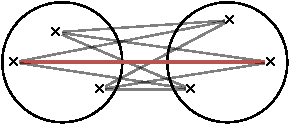
\includegraphics[width=0.55\textwidth]{includes/figures/defi_complete_linkage.pdf}
    \end{center}
\end{defi}

\begin{defi}{Single Linkage}
    \emph{Single Linkage} entspricht der \emph{minimalen} Inter-Cluster-Unterschiedlichkeit.

    Vorgehen:
    \begin{enumerate}
        \item Alle paarweisen Unterschiedlichkeiten zwischen Punkten aus dem ersten und Punkten aus dem zweiten Cluster bestimmen.
        \item Unterschiedlichkeit zwischen beiden Clustern entspricht der \emph{kleinsten Unterschiedlichkeit}.
    \end{enumerate}

    Single Linkage liefert oft unausgewogene Cluster.
    \begin{center}
        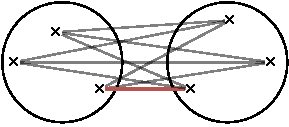
\includegraphics[width=0.55\textwidth]{includes/figures/defi_single_linkage.pdf}
    \end{center}
\end{defi}

\begin{defi}{Average Linkage}
    \emph{Average Linkage} entspricht der \emph{mittleren} Inter-Cluster-Unterschiedlichkeit.

    Vorgehen:
    \begin{enumerate}
        \item Alle paarweisen Unterschiedlichkeiten zwischen Punkten aus dem ersten und Punkten aus dem zweiten Cluster bestimmen.
        \item Unterschiedlichkeit zwischen beiden Clustern entspricht dem \emph{Mittelwert der Unterschiedlichkeit}.
    \end{enumerate}

    \begin{center}
        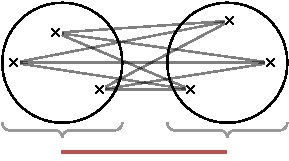
\includegraphics[width=0.55\textwidth]{includes/figures/defi_average_linkage.pdf}
    \end{center}
\end{defi}

\begin{bonus}{K-Means vs Hierarchisches Clustern}
    Clustering Verfahren interpretieren die Daten mit den ihnen impliziten und expliziten Annahmen, wie Cluster zu definieren sind.

    \emph{Hierarchisches Clustern}: Annahme, dass Cluster hierarchisch organisiert sind (d.h. große Cluster setzen sich aus kleineren Clustern zusammen).

    \emph{K-Means Clustering}: Annahme, dass Cluster sphärische Objekte im Feature-Space sind und ungefähr gleich viele Datenpunkte enthalten.
\end{bonus}

\begin{bonus}{Clusteranalyse Hinweise}
    Worauf man achten sollte:
    \begin{enumerate}
        \item Wahl des Unterschiedlichkeitsmaßes (dissimilarity measure)
        \item Vorverarbeitung der Daten
              \begin{itemize}
                  \item Untersuchung, welche Auswirkungen eine Skalierung der Features in Kombination mit der Wahl des Unterschiedlichkeitsmaß (dissimilarity measure) auf Cluster-Ergebnisse hat.
              \end{itemize}
        \item Wahl der Clusteranzahl (oder anderer freier Parameter)
              \begin{itemize}
                  \item Untersuchung, welche Auswirkungen Ihre Wahl einer Clusteranzahl auf Cluster-Ergebnisse hat.
              \end{itemize}
        \item Interpretation der Ergebnisse
              \begin{itemize}
                  \item Cluster-Analyse als Startpunkt einer Untersuchung der Daten, nicht als Endpunkt einer Analyse.
              \end{itemize}
    \end{enumerate}
\end{bonus}